\documentclass[conference]{IEEEtran}
\IEEEoverridecommandlockouts
\usepackage[T1]{fontenc}
\usepackage{amsmath,amssymb,booktabs,array,graphicx}
\usepackage{xcolor}
\usepackage[hidelinks]{hyperref}
\newcommand{\pending}{\textcolor{red!65!black}{Pending}}
\newcommand{\groot}{GR00T N1.7}
\newcommand{\qwen}{Qwen3-VL-2B}
\title{From Stock to Robot-Adapted VLM Backbones: A Frozen-Feature Study on ALOHA and LIBERO-Goal}
\author{\IEEEauthorblockN{Sittipon Kumda\IEEEauthorrefmark{1} and Rachata Pratheep Na Thalang\IEEEauthorrefmark{1}}\IEEEauthorblockA{King Mongkut's Institute of Technology Ladkrabang\\Thailand\\sittiponkumda@gmail.com, pratheepg49@gmail.com}\thanks{\IEEEauthorrefmark{1}These authors contributed equally to this work.}}
\IEEEpubid{\makebox[\columnwidth][l]{\footnotesize 979-8-3195-1044-0/26/\$31.00~\copyright2026 IEEE}\hspace{\columnsep}\makebox[\columnwidth]{}}
\begin{document}
\maketitle
\begin{abstract}
Does a robot-adapted vision--language backbone offer better frozen features
for learning a new manipulation policy than its stock origin? We compare
Qwen3-VL-2B with the related GR00T N1.7 vision--language subtree using matched
action heads within two settings: fixed-instruction, one-view ALOHA
transfer-cube and instruction-conditioned, two-view LIBERO-Goal. ALOHA still
receives a constant text prompt and robot state; it is not an image-only
ablation. At a fixed 100-epoch ALOHA endpoint, three independent training
seeds per backbone yield $49.3\%\pm6.0$ GR00T and $39.8\%\pm11.0$ Qwen
success (mean $\pm$ sample SD), but one seed pair reverses this ordering.
In a separate development-selected LIBERO campaign, two GR00T policies score
84.25\% and 89.00\% on 400 held-out rollouts each; one Qwen
policy scores 91.50\%. In four complete later ALOHA development trajectories,
epoch 250 has higher validation flow loss than epoch 50, but rollout success
improves in three and ties in one. The adapted endpoint is not consistently
ahead across these policy runs. The lineage includes intermediate adaptation, and
the two tasks differ in more than instruction variation; neither robot
pretraining alone nor a language-specific effect is isolated.
\end{abstract}
\begin{IEEEkeywords}
vision--language--action, robot learning, frozen representations, evaluation,
imitation learning
\end{IEEEkeywords}

\section{Introduction}
Vision--language--action policies connect visual and language representations
to robot actions. OpenVLA, $\pi_0$, and GR00T N1 demonstrate integrated
policies learned from robot data~\cite{openvla,pi0,grootn1}. When a user
trains a new controller, however, a practical choice is whether to start
from a stock VLM or its robot-adapted descendant while keeping the backbone
frozen. The potential benefit could lie in features useful for control,
yet a stronger complete robot policy would not by itself show that its
frozen VLM features transfer better. Component studies also show that
backbone, architecture, and data choices interact~\cite{robovlms}. We
therefore compare the frozen features under matched downstream heads.

We compare \qwen{} with the vision--language subtree extracted from \groot{}.
The released lineage includes Cosmos-Reason2-2B between these endpoints
\cite{groot17}. The comparison asks whether the \emph{released robot-adapted
endpoint} helps a new action head relative to the stock endpoint. It cannot
attribute any difference to the final robot-training stage rather than
intermediate adaptation, architecture, or processing changes.

Two questions organize the study. \textbf{RQ1:} with a newly trained action
head, does the robot-adapted endpoint outperform its stock origin in a
fixed-instruction manipulation task or in instruction-conditioned tasks,
and does that contrast persist across independent training seeds?
\textbf{RQ2:} what do behavioral failures, text-token controls, and offline
validation reveal---or fail to reveal---about the closed-loop contrast?
ALOHA transfer-cube is a single fixed-instruction bimanual handover~\cite{aloha};
LIBERO-Goal has ten instruction-conditioned single-arm goals~\cite{libero}.
ALOHA's constant prompt does not distinguish target tasks, but the model
still receives text, images, and robot state. The benchmarks also differ in
embodiment, cameras, actions, and training, so this is not a controlled
image-only-versus-language intervention.

Our contribution is a matched-head endpoint comparison with explicit
training-run replication, paired ALOHA scene analysis, behavioral diagnostics,
and a checkpoint-level view of offline metrics alongside development success.
The result is conditional: the advantage changes by seed and setting; offline
metric rankings also depend on the measure selected.
We separate three evidence sources: the submitted observations, a prospective
fixed-endpoint ALOHA study, and a later development-selected campaign with
final LIBERO evaluations and sparse ALOHA checkpoint measurements. They differ
in training, selection, and evaluation, so their success rates are not pooled.
Training seeds index independent learned heads; checkpoint measurements and
additional rollout scenes do not constitute new training runs.

\IEEEpubidadjcol
\section{Related Work}
\textbf{VLA design studies.} RoboVLMs studies backbone, architecture, and data
choices across more than 600 experiments~\cite{robovlms}; OpenVLA, $\pi_0$, and
GR00T N1 study integrated robot policies~\cite{openvla,pi0,grootn1}. Our smaller
component study removes the released action expert and compares frozen features
using a shared downstream recipe within each benchmark. It does not evaluate
the complete GR00T policy or establish interactions across a broad model family.

\textbf{Observation configuration.} Hand-centric views can affect learning and
generalization~\cite{handview}. The later campaign uses two-camera LIBERO only.
Its excluded one-camera condition does not support a camera-count conclusion.
Our cross-benchmark comparisons also change embodiment and action space, so
they do not isolate a single factor.

\textbf{Evaluation validity.} Critical Interval MSE studies offline validation
focused on task-critical segments~\cite{cimse}. We examine selected aggregate
losses and diagnostics, without testing that method or claiming that all offline
evaluators fail. LIBERO-PRO reports sensitivity to evaluation conditions and
instruction perturbations~\cite{liberopro}. The submitted fixed-instruction ALOHA ablation cautions that sensitivity to
removing text tokens need not imply task-discriminative language use.

\section{Experimental Design}
\subsection{Frozen endpoints and downstream heads}
Both endpoints are read at language layer 16. This is the retained final layer
for the extracted GR00T backbone and an intermediate read for the stock model.
The latter receives its language stack's final RMS normalization at that read.
This controls the specific final-versus-intermediate normalization discrepancy;
it does not make the released systems identical or isolate a single pretraining
dataset. Processor settings, view order, token padding, and read depth are
matched within each benchmark and recorded with the feature cache.
In the revised path, processor-masked padding is removed and real tokens are
right-padded with zeros to a fixed budget, avoiding batch-dependent pad features.

The backbone is frozen and its image/text features are cached. Only a token
adapter and a DiT-style~\cite{dit} flow-matching~\cite{flow} action head train.
The adapter supplies conditioning
and tokens to a transformer decoder. Given demonstrated actions $a$, Gaussian
noise $\epsilon$, and $t\sim\mathcal U(0,1)$, the loss is
\begin{equation}
 \mathcal L=\mathbb E\left[\left\|v_\theta((1-t)\epsilon+ta,t,c)
                    -(a-\epsilon)\right\|_2^2\right].
\end{equation}
The new heads are matched between endpoints within each benchmark. They are
\emph{not} identical across benchmarks: the inspected configurations contain
19,165,319 trainable parameters for two-camera LIBERO and 14,014,990 for ALOHA.
Both predict 16 actions and execute eight before replanning, with three
integration steps at inference. The configurations use decoder widths 320 and
256, respectively. These differences limit cross-benchmark interpretation.

\subsection{Demonstrations and validation}
ALOHA provides a single top-camera view, robot state, and the same
transfer-cube instruction on every demonstration and rollout. LIBERO-Goal
provides agent and wrist views, robot state, and task-varying instructions.
Within a benchmark both endpoints receive the same observation specification.
Across benchmarks, instruction variability changes together with embodiment,
views, action space, and head size; their results cannot isolate the effect
of text or of a visual feature alone.

The revised protocol holds out whole demonstration episodes. A deterministic
split with seed 42 assigns ten percent of episodes from each LIBERO task to
validation, with at least one held-out episode per task. For ALOHA's 50
demonstrations, 45 train and five validate. All frames and action chunks from
an episode remain in that split; chunks are padded only within their episode.
The same split is shared across backbones, training seeds, and camera controls.

ALOHA state and absolute joint targets use mean/std statistics computed from
training episodes only. The same statistics are used offline and in the simulator,
with predicted actions denormalized before execution. LIBERO retains its raw
end-effector delta actions and recorded state representation. Validation loss
measures demonstrated action prediction on held-out episodes; test success
measures the policy's behavior under its own actions in simulation. The two
quantities are not interchangeable.

\subsection{Training campaigns and selection}
The fixed-endpoint ALOHA study uses three independent head-training seeds,
3--5, per backbone, controlling initialization, shuffling, dropout, and flow
noise. Its locked recipe uses AdamW, weight decay $10^{-2}$, warmup--cosine
scheduling, decoder peak learning rate $3\times10^{-4}$, half that rate for the
adapter, batch size 256, and a fixed epoch-100 checkpoint. It differs from the
submitted recipe; it is a prospective comparison rather than an exact reproduction.

The later campaign uses development-rollout success for checkpoint selection.
The final LIBERO checkpoints are GR00T seed 3 at epoch 100 (44,800 updates),
Qwen seed 3 at epoch 130 (58,240), and GR00T seed 4 at epoch 110 (49,280
updates). These are selected endpoints with unequal training budgets, not an
equal-update ablation. The ALOHA sparse sweep evaluates existing checkpoints
for a separate development analysis.

\subsection{Validation metrics}
For $N$ held-out state/action chunks of horizon $H$ and dimension $D$, action
MSE and MAE average $(\hat a-a)^2$ and $|\hat a-a|$, respectively, over all
$NHD$ entries. Flow loss averages the squared velocity residual in (1), with
Gaussian noise and uniformly sampled flow time. Validation fixes RNG seed 4242.
Action prediction uses three integration steps and batch sampling seeds
$424200+b$ for validation batch $b$; it samples a generated action chunk rather
than evaluating the demonstrated velocity target alone. Sampling is isolated
from the flow-loss RNG stream.

LIBERO metrics use the configured raw action representation (seven dimensions);
ALOHA metrics use configured normalized joint-target space (14 dimensions),
with training-only mean/std and denormalization before execution. Thus their
absolute losses cannot be compared across benchmarks. The later LIBERO records
contain $N=6238$ validation chunks and ALOHA $N=2000$. These are overlapping
within-episode samples, not thousands of independent demonstrations. The saved
split manifests contain 450/50 train/validation LIBERO episodes and 45/5 ALOHA
episodes with full, disjoint membership.

\subsection{Evaluation pairing and uncertainty}
The fixed-endpoint ALOHA study evaluates each policy on 200 shared scene IDs,
10000--10199, within each training-seed pair, with matched environment and
policy-sampling seeds. It saves no videos or traces and sets offscreen
antialiasing samples to zero; camera images are still rendered for the policy.
The later sparse ALOHA sweep uses 50 development starts, IDs 20000--20049.
The evaluator resets with $(\mathrm{episode\ index}+\mathrm{seed\ offset})137+42$,
independent of backbone, and records state/image fingerprints before actions.
The sparse sweep is summarized descriptively; no paired significance test is
claimed for its checkpoint comparisons. The exported checkpoint digest,
episode count, epoch, optimizer step, and loss-history binding are retained
for each measured point; 37 of 54 requested positions have verified results.

LIBERO final evaluation uses 40 starts per task for ten tasks (400 total),
separate from the ten development starts per task. Seed-3 initial-state and
initial-observation fingerprints match for all 400 backbone pairs. This verifies
physical-start pairing, not independent training replication. We report marginal
success rates for these policies without inferring a paired significance test
from marginal totals.

We report one success rate per independent trained head and unweighted means
and sample SD across heads. An SD for one seed is unavailable. Conditional
rollout uncertainty and paired episode tests do not quantify variation over
unseen training seeds or tasks. The fixed-endpoint ALOHA analysis uses exact
two-sided McNemar tests on each matched seed pair, with Holm correction across
the three comparisons. These tests describe rollout variation conditional on
the trained policies, not variation from retraining.

\section{Backbone Transfer in Two Task Settings}
\subsection{Fixed-instruction ALOHA}
The submitted paper reported 245/400 GR00T successes and 207/400 Qwen
successes (61.25\% and 51.75\%) across two reported runs per backbone. These
historical summaries are kept separate from both later campaigns because their
training and evaluation protocols differ.

\paragraph{Fixed-endpoint ALOHA study.}
A separate study reports six independently trained policies, each trained
for 100 epochs and evaluated on 200 matched starts within each training-seed pair.
Table~\ref{tab:aloha-matched}
reports Qwen3-VL minus GR00T. The six local per-episode test records and the
regenerated paired analysis were checked against these counts; the older
submitted campaign's training provenance remains separate.
Mean success across the three training seeds was
49.3\% $\pm$ 6.0 for GR00T and 39.8\% $\pm$ 11.0 for Qwen3-VL; the mean paired
difference was $-9.5\pm16.9$ points (sample SD across seeds). GR00T led in seeds
4 and 5, while Qwen3-VL led in seed 3. These seed means are descriptive at
$n=3$; the paired rollout tests are conditional on each trained policy pair.

\begin{table*}[t]
\centering\small\setlength{\tabcolsep}{7pt}
\caption{Fixed-epoch-100 ALOHA comparison on the same 200 starts per seed.
Q only / G only counts starts on which only one policy succeeds; these
paired counts explain the success gap. $p$ is an exact paired test adjusted
across the three seed comparisons.}
\label{tab:aloha-matched}
\begin{tabular}{@{}crrrcc@{}}
\toprule
Seed & GR00T & Qwen & $Q-G$ (pp) & Q only / G only & Adjusted $p$ \\
\midrule
3 & 85/200 (42.5\%) & 104/200 (52.0\%) & $+9.5$ & 52 / 33 & 0.05025 \\
4 & 107/200 (53.5\%) & 61/200 (30.5\%) & $-23.0$ & 20 / 66 & $2.00\times10^{-6}$ \\
5 & 104/200 (52.0\%) & 74/200 (37.0\%) & $-15.0$ & 27 / 57 & 0.00281 \\
\bottomrule
\end{tabular}
\end{table*}

The matched-start counts favor Qwen in seed 3 and GR00T in seeds 4 and 5;
the adjusted seed-3 test is inconclusive. The three-seed mean difference
equals the submitted 9.5-point gap, but its absolute rates are about
11.9 points lower. Because
training budget, normalization, head configuration, seeds, and evaluation
rendering changed, these rates are not an exact reproduction and do not identify
why the absolute level differs.

\paragraph{Later sparse development sweep.}
The exported sweep completes 37 checkpoint evaluations among 54 requested
positions, including six epoch-zero positions without saved checkpoints.
It covers GR00T seeds 3--5 and Qwen seeds 3--4, with 50 development starts
per measured checkpoint. Missing positions are unmeasured, not failures.
Four trajectories (both backbones, seeds 3--4) have verified checkpoints
at both epochs 50 and 250. Fig.~\ref{fig:aloha-dynamics} compares those
predefined first and final measured endpoints: training loss falls and
validation flow loss nearly doubles in all four, but development success
rises in three and stays level in one. For GR00T seed 4, success changes
from 1/50 to 29/50 while validation loss changes from 0.209 to 0.394.
This is a concrete mismatch for these checkpoints, not a held-out test of
which selection rule generalizes. The other 29 verified probes remain
development measurements from dependent training trajectories.

\begin{figure*}[t]
\centering
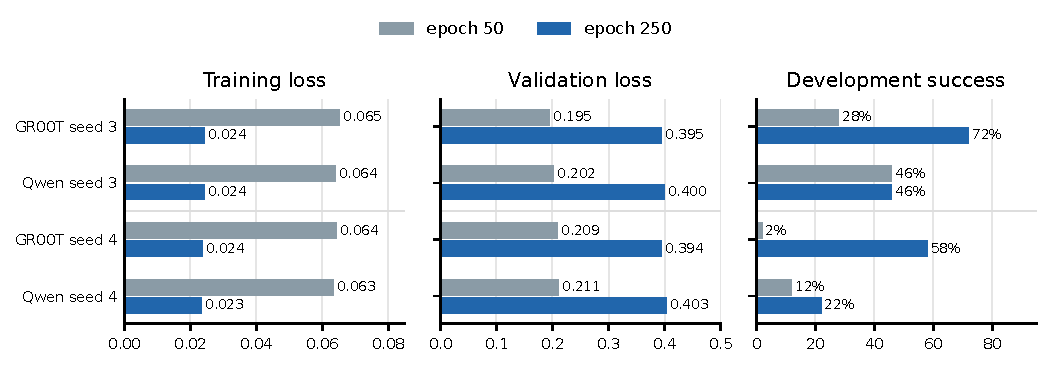
\includegraphics[width=.96\textwidth]{figures/aloha_epoch50_vs250.pdf}
\caption{First versus final measured checkpoints in the four complete
ALOHA development trajectories. Losses use held-out demonstration episodes;
success uses the same 50 development starts at each checkpoint. Values are
from saved same-epoch records, with no interpolation or post-hoc choice of
the best success checkpoint. These are dependent checkpoints, not four new
training runs or held-out final tests.}
\label{fig:aloha-dynamics}
\end{figure*}

\subsection{Instruction-conditioned LIBERO-Goal}
The separate, development-selected LIBERO campaign gives a narrower
comparison. GR00T succeeds on 337/400 held-out starts in seed 3 (epoch 100,
44,800 updates) and 356/400 in seed 4 (epoch 110, 49,280 updates). Qwen
succeeds on 366/400 in seed 3 (epoch 130, 58,240 updates). Thus, the only
matched training-seed comparison favors Qwen by 29/400 starts, or 7.25
percentage points. This contrast is conditional on the two selected policies:
their training budgets differ, and the final sample has two GR00T policies
and one Qwen policy. The GR00T two-seed mean is 86.625\% (sample SD 3.359
points); a comparable Qwen across-seed estimate is unavailable.

Fig.~\ref{fig:libero-tasks} shows how the seed-3 gap is distributed across
the ten goals. Qwen has more successes on five tasks, GR00T on two, and
the policies tie on three. Tasks 0, 3, and 9 contribute 26 of the net 29
additional Qwen successes; other task differences partly offset each other.
The plot is a breakdown of the same 400 starts per policy, not ten
independent backbone replications. Task-level marginal counts also do not
identify which individual paired starts changed outcome.

\begin{figure}[t]
\centering
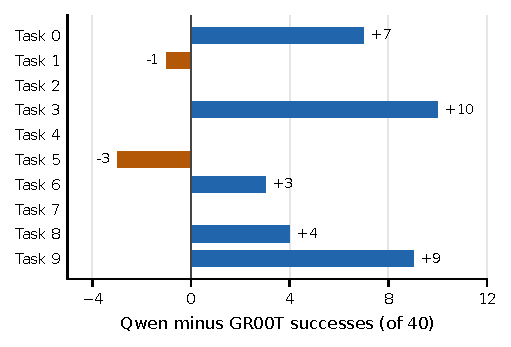
\includegraphics[width=\columnwidth]{figures/libero_seed3_task_difference.pdf}
\caption{Held-out LIBERO-Goal success difference by task for the selected
seed-3 policies. Each task has 40 starts per backbone; positive bars favor
Qwen and negative bars favor GR00T. The bars sum to Qwen's 29/400 overall
advantage. These are marginal task counts, and the selected policies had
different training budgets.}
\label{fig:libero-tasks}
\end{figure}

\paragraph{Answer to RQ1.}
In the fixed-endpoint ALOHA study the robot-adapted endpoint leads in two
of three seed pairs and has the higher mean; the third pair favors stock
Qwen. The later LIBERO held-out seed-3 pair also favors Qwen, with final
training-run counts of two GR00T and one Qwen. These observations do not
establish a consistent advantage for the robot-adapted endpoint. The contrast between settings
does not establish that instruction variation causes the change in ordering.

\subsection{Observed receiving-gripper failures}
In the submitted analysis, contact rates were 89.2\%/92.5\%, yet handover
given lift was 71.6\%/59.7\% (GR00T/Qwen). The gap appears after lift,
not at first contact; these conditional summaries are descriptive.

Instrumented ALOHA rollouts recorded states, commands, staged rewards, and
per-replan attention on a separate 200-start cohort per endpoint.
Table~\ref{tab:failures} accounts for every lifted episode in that trace
cohort. The receiver never opened in
25/173 lifted GR00T episodes and 45/172 lifted stock episodes. This is an
observed failure pattern, not proof that pretraining caused improved visual
reasoning. Historical classification used endpoint-specific opening thresholds
(0.655 and 0.647), so it remains descriptive. The new matched evaluation saved
no commanded or observed gripper traces and cannot validate this mechanism.
The final category is renamed operationally: a gripper that opens
and closes without completing transfer need not have ``closed on nothing.''

\begin{table}[t]
\centering\small\setlength{\tabcolsep}{4pt}
\caption{Observed receiving-gripper outcome after lift in the separate
submitted trace cohort. Each column sums to its lifted total; rates use
that column's denominator.}
\label{tab:failures}
\begin{tabular}{@{}lrr@{}}
\toprule
Observed receiver behavior & GR00T & Qwen3-VL \\
\midrule
Never opened & 25 (14.5\%) & 45 (26.2\%) \\
Opened, did not close & 23 (13.3\%) & 16 (9.3\%) \\
Opened/closed, no transfer & 4 (2.3\%) & 8 (4.7\%) \\
Transferred & 121 (69.9\%) & 103 (59.9\%) \\
\midrule
Total lifted & 173 & 172 \\
\bottomrule
\end{tabular}
\end{table}

The trace cohort is separate from the matched 100-epoch study, so its
categories cannot explain that study's success gap. Attention and
proprioceptive probes do not establish an exclusively visual mechanism.
No intervention repaired the opening command while holding the rest of
the policy fixed.

\section{Conditioning and Offline Diagnostics}
\subsection{Offline rankings}
\textbf{The offline ranking disagreement is metric-dependent.} In the later
LIBERO seed-3 final comparison (Table~\ref{tab:metrics}), GR00T has lower flow
loss and lower MAE, yet lower closed-loop success. Action MSE instead favors
Qwen and agrees with the success ordering. This single paired endpoint contrast
does not estimate predictive calibration or correlation across a population of
policies, nor show that all offline metrics are uninformative.

\begin{table}[t]
\centering\small\setlength{\tabcolsep}{3pt}
\caption{What each measure would favor for the completed LIBERO seed-3 pair.
Offline measures use the same 6238 validation chunks (lower is better);
held-out success uses 400 starts per policy (higher is better).}
\label{tab:metrics}
\begin{tabular}{@{}lrrl@{}}\toprule
Measure & GR00T & Qwen & Favors\\\midrule
Flow loss & 0.1404 & 0.1550 & GR00T\\
Action MAE & 0.0760 & 0.0766 & GR00T\\
Action MSE & 0.0361 & 0.0358 & Qwen\\
\midrule
Final success & 84.25\% & 91.50\% & Qwen\\\bottomrule
\end{tabular}
\end{table}

In the fixed-endpoint ALOHA study, GR00T has lower validation flow loss in
all three seed pairs, yet Qwen wins the seed-3 rollout comparison. In the
separate development sweep (Fig.~\ref{fig:aloha-dynamics}), epoch 250 has
higher validation loss than epoch 50 for all four complete trajectories,
although success improves in three and ties in one. These are observed
counterexamples to always selecting the lower-loss policy; the development
probes do not establish how well either selection rule generalizes.

\subsection{A task-critical measure still to test}
In the submitted trace cohort, the receiver never opens in 45/172 lifted
Qwen episodes versus 25/173 GR00T episodes. An aggregate action loss over
all chunks and 14 dimensions does not report error specifically at this
event. We did not compute a post-lift gripper metric on the same cohort,
so cannot say it would predict success. Critical-interval validation
\cite{cimse} is a concrete method to test this hypothesis.

This is a proxy-metric caution, not a claim about emergent scaling
\cite{emergent}. Neither attention nor feature similarity is a calibrated
success predictor in this study.

\subsection{Historical fixed-instruction language control}
In the submitted diagnostics, zeroing text tokens raises flow loss by factors
of 1.14 for GR00T and 1.24 for Qwen on fixed-instruction ALOHA, versus 6.12
and 5.39 on two-camera LIBERO. The ALOHA control shows that token removal can
perturb conditioning even when text does not distinguish tasks. Larger LIBERO
ratios are consistent with instruction dependence, but do not establish semantic
understanding. This intervention is out of distribution; the ALOHA ratio is not
a universal perturbation floor that can be subtracted from LIBERO. Together
with the receiving-gripper observations, these diagnostics suggest where to
probe the policies, but do not show how backbone adaptation caused their
different success rates.

\section{Limitations}
This study evaluates two frozen endpoints in one lineage. The endpoint contrast
combines intermediate adaptation with robot training; it does not isolate one
pretraining dataset or stage. Cosmos-Reason2 intermediate controls, other
backbone families, Qwen3.5-0.8B capacity controls, full-backbone fine-tuning,
more seeds, diverse tasks, and physical robots are not completed here. No
training cost or cost--benefit tradeoff is measured. ALOHA uses a constant
text prompt, and the across-benchmark contrast changes several variables at once;
the present design cannot estimate the causal value of adding instructions.

The fixed-endpoint ALOHA study has three independent seeds per backbone, and
the later LIBERO final campaign has two GR00T seeds and one Qwen seed. Such
small samples give imprecise training-variation estimates. The sparse ALOHA
sweep is incomplete and developmental, with dependent checkpoint measurements.
The fixed-endpoint ALOHA test outcomes are retained locally for all six
policies and support regenerated paired statistics. The older submitted
campaign's training provenance is less complete. The latest ALOHA sweep
provides verified checkpoint-level development measurements. Different
campaigns cannot be pooled to increase the apparent replication count.

Whole-episode validation prevents frame leakage between train and validation,
but one fixed split and few ALOHA validation episodes limit coverage.
Development/final scene separation does not verify that all final scene poses
are absent from the demonstrations. Head, normalization, budget, and rendering
differences constrain cross-campaign comparisons. Stage rates, attention, and
gripper categories are descriptive rather than causal, and nonsignificance
does not establish equivalence.

\section{Conclusion}
Our motivating choice is whether to reuse a stock VLM backbone or its
robot-adapted descendant when fitting a new manipulation action head. In
fixed-instruction ALOHA, the three-seed fixed-endpoint mean favors GR00T by
9.5 points, but one seed reverses direction. In instruction-conditioned
LIBERO-Goal, the held-out seed-3 pair favors Qwen, with unequal
selected training budgets and a final sample of two GR00T heads and one Qwen
head. These observations do not establish a setting-independent benefit of the adapted endpoint or
attribute the cross-task contrast to language variation. At epoch 250,
validation flow loss exceeds epoch 50 in all four complete ALOHA development
trajectories, but success improves in three and ties in one. LIBERO flow
loss and MAE disagree with the seed-3 rollout ordering, whereas MSE agrees.
Historical receiving-gripper failures and text-token controls motivate
targeted tests rather than establish a mechanism. The next decisive
experiments are matched final seeds and within-benchmark text controls,
followed by the intermediate lineage checkpoint.

\begin{thebibliography}{13}
\bibitem{openvla} M. J. Kim et al., ``OpenVLA: An open-source vision-language-action
model,'' arXiv:2406.09246, 2024.
\bibitem{pi0} K. Black et al., ``$\pi_0$: A vision-language-action flow model for
general robot control,'' arXiv:2410.24164, 2024.
\bibitem{grootn1} NVIDIA, ``GR00T N1: An open foundation model for generalist
humanoid robots,'' arXiv:2503.14734, 2025.
\bibitem{groot17} NVIDIA, ``GR00T-N1.7-3B,'' released model card and configuration,
\url{https://huggingface.co/nvidia/GR00T-N1.7-3B}, accessed Oct. 21, 2026.
\bibitem{robovlms} X. Li et al., ``What matters in building vision--language--action
models for generalist robots,'' \emph{Nature Machine Intelligence}, vol. 8,
pp. 158--172, 2026, doi: 10.1038/s42256-025-01168-7.
\bibitem{aloha} T. Z. Zhao, V. Kumar, S. Levine, and C. Finn, ``Learning fine-grained
bimanual manipulation with low-cost hardware,'' in \emph{Proc. RSS}, 2023.
\bibitem{libero} B. Liu et al., ``LIBERO: Benchmarking knowledge transfer for
lifelong robot learning,'' in \emph{NeurIPS Datasets and Benchmarks}, 2023.
\bibitem{handview} K. Hsu, M. J. Kim, R. Rafailov, J. Wu, and C. Finn,
``Vision-based manipulators need to also see from their hands,''
in \emph{Proc. ICLR}, 2022.
\bibitem{cimse} H. Huang, T. Zheng, Y. Chen, J. You, and Y. Gao, ``Critical interval
MSE: Toward reliable offline validation for robot manipulation policies,''
arXiv:2606.29898, 2026.
\bibitem{liberopro} X. Zhou, Y. Xu, G. Tie, Y. Chen, G. Zhang, D. Chu, P. Zhou,
and L. Sun, ``LIBERO-PRO: Towards robust and fair evaluation of vision-language-action
models beyond memorization,'' arXiv:2510.03827, 2025.
\bibitem{dit} W. Peebles and S. Xie, ``Scalable diffusion models with transformers,''
in \emph{Proc. ICCV}, 2023.
\bibitem{flow} Y. Lipman, R. T. Q. Chen, H. Ben-Hamu, M. Nickel, and M. Le,
``Flow matching for generative modeling,'' in \emph{Proc. ICLR}, 2023.
\bibitem{emergent} J. Wei et al., ``Emergent abilities of large language models,''
\emph{Transactions on Machine Learning Research}, 2022.
\end{thebibliography}
% Fail compilation if this draft grows beyond the conference's six-page limit.
% clearpage flushes the last content page, so the next-page counter is at most 7.
\clearpage
\ifnum\value{page}>7
  \PackageError{camera-ready}{Manuscript exceeds six pages}{Reduce content without changing the conference layout.}
\fi
\end{document}
